\section{The Postconciliar Roman Sanctuary}
Every object gathered in a Catholic sanctuary serves the one sacrifice of Christ made present upon the altar and the proclamation of the Word of God that prepares the faithful to share in it. From the freestanding stone mensa and the stationary ambo to the smallest linen purificator, the Roman Rite arranges physical matter with quiet clarity so that the eye recognizes what the Church celebrates without distraction. The plates that follow present forty principal furnishings, vessels, linens, books, service articles, and vestments of the postconciliar Roman sanctuary in monochrome graphite, separating universal Roman law from United States territorial adaptations and comparing each item directly with its counterpart in the 1962 Roman Missal.

\PCDPlateHeader{Plate I --- The Postconciliar Roman Sanctuary}{Not to common scale (architectural perspective)}
\ifdefined\TriptychPrintEdition
\begin{center}
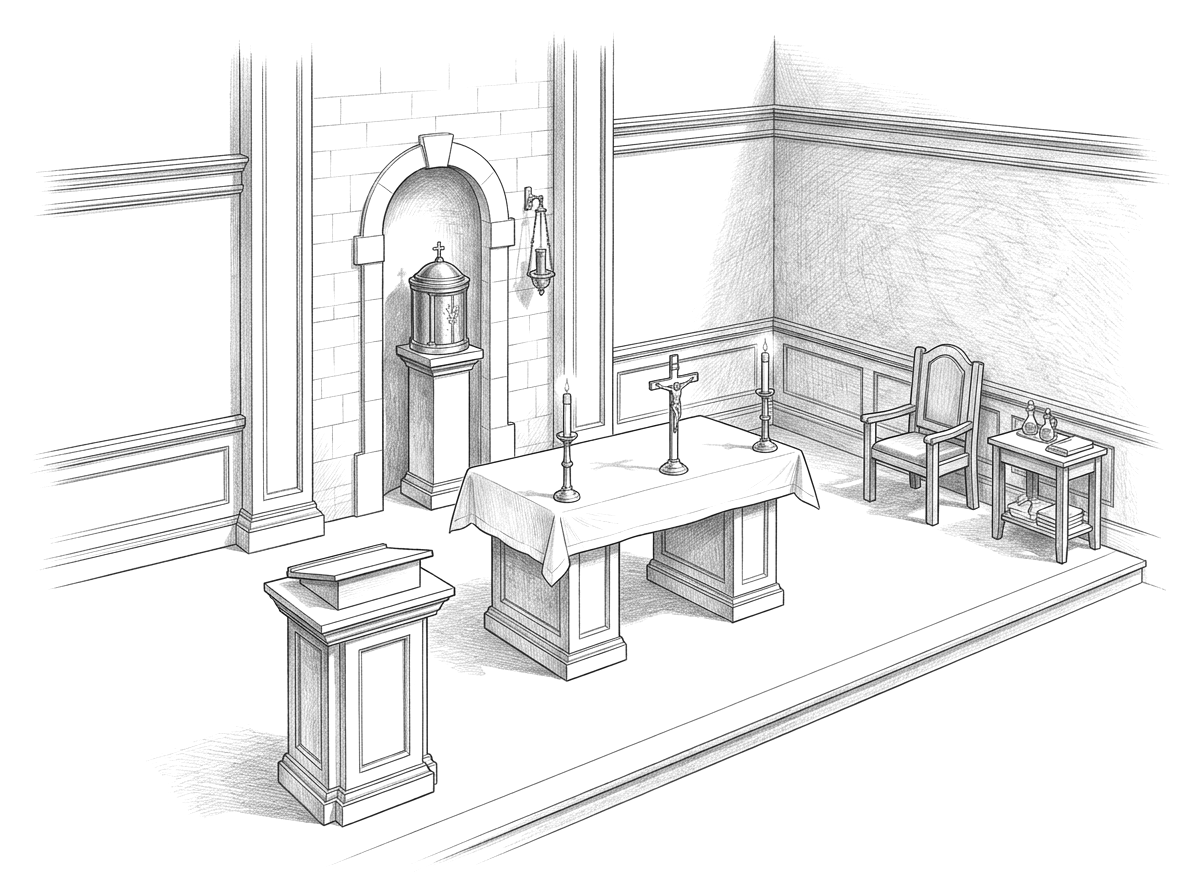
\includegraphics[width=0.96\linewidth,height=4.25in,keepaspectratio]{liturgy/roman-rite/postconciliar/2008-latin-2011-us-english/reference/roman-sanctuary-dictionary/shared/artwork/graphite/pc-art-01-sanctuary-composition.png}
\end{center}
\PCDPositionKey{Center: freestanding Altar with white Altar Cloth, two Altar Candles, and Altar Cross with corpus; foreground left: stationary Ambo; rear recessed niche: solid locked Tabernacle with hanging Sanctuary Lamp; rear right: Presidential Chair beside Credence Table holding cruets and linens.}
\else
\textbf{Visual Plate Summary (Plate I --- The Postconciliar Roman Sanctuary, Not to common scale (architectural perspective)):} Full architectural monochrome graphite perspective of a postconciliar Roman Catholic sanctuary showing the spatial coordination of freestanding stone altar dressed in white cloth with two candles and crucifix, permanent stone ambo in left foreground, wooden presidential chair and credence table with glass cruets and folded linens on the right, and a solid architectural tabernacle on a pillar inside a recessed arched niche with a hanging sanctuary lamp beside it. No altar cards, gradines, or rail appear.

\textbf{Reading order and object placement:} Center: freestanding Altar with white Altar Cloth, two Altar Candles, and Altar Cross with corpus; foreground left: stationary Ambo; rear recessed niche: solid locked Tabernacle with hanging Sanctuary Lamp; rear right: Presidential Chair beside Credence Table holding cruets and linens.
\fi

Look first across the whole sanctuary in Plate I. In the postconciliar Roman arrangement (GIRM 296--318), the architectural focus is clear and uncluttered: the freestanding altar stands at the center so that ministers may move around it and celebrate facing the congregation where possible (GIRM 299); the stationary ambo announces the dignity of the Liturgy of the Word (GIRM 309); the presidential chair expresses the priest's office of presiding and leading prayer without resembling a throne (GIRM 310); the credence table holds vessels and linens off the mensa until the Preparation of the Gifts (GIRM 118c, 306); and the solid, locked tabernacle with its continuously burning oil or wax lamp honors the Eucharistic Reservation apart from the altar of celebration (GIRM 314--316).

\subsection*{Reading the Status Tags}
Each entry names its status for the 2008 Latin third typical edition of the Roman Missal as implemented in the 2011 United States edition (as of 2026-11-25). \PCDTag{required} marks an item prescribed by universal Roman law; \PCDTag{provided} marks an item expressly appointed for a rite, ministry, or occasion; \PCDTag{permitted} and \PCDTag{optional} mark lawful choices governed by rubric or celebrant judgment; \PCDTag{territorial adaptation} marks a norm established by the United States Conference of Catholic Bishops; \PCDTag{customary} marks widespread parish practice distinct from universal prescription; and \PCDTag{superseded} appears exclusively in the chronological historical section.

\subsection*{Monochrome Key for Liturgical Vestment Colors}
In monochrome graphite plates, vestment and textile colors appointed in the General Instruction of the Roman Missal (no.~346, with United States adaptations) are named in words and keyed below rather than encoded by tint alone.

\ifdefined\TriptychPrintEdition
{\footnotesize\begin{longtable}{>{\raggedright\arraybackslash}p{0.14\linewidth}>{\raggedright\arraybackslash}p{0.27\linewidth}>{\raggedright\arraybackslash}p{0.52\linewidth}}
\toprule
\textbf{Color} & \textbf{Monochrome key} & \textbf{Appointed occasions (US 2011 GIRM 346)} \\
\midrule
\endhead
\textbf{White} & \tikz[baseline=-0.5ex]{\draw[black,line width=0.5pt,fill=white] (0,0) rectangle (0.34cm,0.22cm);}\ Open white box (unshaded) & Easter Time, Christmas Time, celebrations of the Lord (except Passion), Blessed Virgin Mary, Angels, non-martyr Saints, All Saints, St. John the Baptist, St. John the Evangelist, Chair of St. Peter, Conversion of St. Paul; also permitted in the United States for funeral Masses (US GIRM 346e). \\
\textbf{Red} & \tikz[baseline=-0.5ex]{\draw[black,line width=0.5pt] (0,0) rectangle (0.34cm,0.22cm); \draw[black,line width=0.35pt] (0.06cm,0)--(0.06cm,0.22cm) (0.12cm,0)--(0.12cm,0.22cm) (0.18cm,0)--(0.18cm,0.22cm) (0.24cm,0)--(0.24cm,0.22cm) (0.29cm,0)--(0.29cm,0.22cm);}\ Vertical parallel rule & Palm Sunday of the Passion of the Lord, Good Friday, Pentecost Sunday, celebrations of the Passion of the Lord, birthdays (martyrdoms) of Apostles and Evangelists, and celebrations of Martyr Saints (GIRM 346b). \\
\textbf{Green} & \tikz[baseline=-0.5ex]{\draw[black,line width=0.5pt] (0,0) rectangle (0.34cm,0.22cm); \draw[black,line width=0.35pt] (0,0.12cm)--(0.10cm,0.22cm) (0,0.02cm)--(0.20cm,0.22cm) (0.08cm,0)--(0.30cm,0.22cm) (0.18cm,0)--(0.34cm,0.16cm) (0.28cm,0)--(0.34cm,0.06cm);}\ Diagonal rising hatch & Offices and Masses of Ordinary Time (GIRM 346c). \\
\textbf{Violet} & \tikz[baseline=-0.5ex]{\draw[black,line width=0.5pt] (0,0) rectangle (0.34cm,0.22cm); \draw[black,line width=0.3pt] (0,0.11cm)--(0.11cm,0.22cm) (0,0)--(0.22cm,0.22cm) (0.11cm,0)--(0.33cm,0.22cm) (0.22cm,0)--(0.34cm,0.12cm) (0,0.11cm)--(0.11cm,0) (0,0.22cm)--(0.22cm,0) (0.11cm,0.22cm)--(0.33cm,0) (0.22cm,0.22cm)--(0.34cm,0.10cm);}\ Cross-hatched grid & Advent and Lent; also lawful for Offices and Masses for the Dead (GIRM 346d). \\
\textbf{Black} & \tikz[baseline=-0.5ex]{\draw[black,line width=0.5pt,fill=black] (0,0) rectangle (0.34cm,0.22cm);}\ Solid black fill & Permitted where customary (including in the United States) for Masses for the Dead (US GIRM 346e). \\
\textbf{Rose} & \tikz[baseline=-0.5ex]{\draw[black,line width=0.5pt] (0,0) rectangle (0.34cm,0.22cm); \fill[black] (0.06cm,0.055cm) circle (0.4pt) (0.13cm,0.055cm) circle (0.4pt) (0.20cm,0.055cm) circle (0.4pt) (0.27cm,0.055cm) circle (0.4pt) (0.095cm,0.11cm) circle (0.4pt) (0.165cm,0.11cm) circle (0.4pt) (0.235cm,0.11cm) circle (0.4pt) (0.06cm,0.165cm) circle (0.4pt) (0.13cm,0.165cm) circle (0.4pt) (0.20cm,0.165cm) circle (0.4pt) (0.27cm,0.165cm) circle (0.4pt);}\ Fine stippled dots & Permitted where customary on Gaudete Sunday (Third Sunday of Advent) and Laetare Sunday (Fourth Sunday of Lent) (GIRM 346f). \\
\textbf{Gold or Silver} & \tikz[baseline=-0.5ex]{\draw[black,line width=0.6pt] (0,0) rectangle (0.34cm,0.22cm); \draw[black,line width=0.3pt] (0.04cm,0.04cm) rectangle (0.30cm,0.18cm);}\ Double-bordered festive frame & Festive vestments may be worn on more solemn occasions even if not of the color of the day (GIRM 346g); in the United States, gold- or silver-colored vestments are permitted on more solemn occasions (US GIRM 346h). \\
\bottomrule
\end{longtable}}
\else
{\footnotesize\begin{longtable}{>{\raggedright\arraybackslash}p{0.14\linewidth}>{\raggedright\arraybackslash}p{0.25\linewidth}>{\raggedright\arraybackslash}p{0.54\linewidth}}
\toprule
\textbf{Color} & \textbf{Print pattern key} & \textbf{Appointed occasions (US 2011 GIRM 346)} \\
\midrule
\endhead
\textbf{White} & Open white box (unshaded) & Easter Time, Christmas Time, celebrations of the Lord (except Passion), Blessed Virgin Mary, Angels, non-martyr Saints, All Saints, St. John the Baptist, St. John the Evangelist, Chair of St. Peter, Conversion of St. Paul; also permitted in the United States for funeral Masses (US GIRM 346e). \\
\textbf{Red} & Vertical parallel rule & Palm Sunday of the Passion of the Lord, Good Friday, Pentecost Sunday, celebrations of the Passion of the Lord, birthdays (martyrdoms) of Apostles and Evangelists, and celebrations of Martyr Saints (GIRM 346b). \\
\textbf{Green} & Diagonal rising hatch & Offices and Masses of Ordinary Time (GIRM 346c). \\
\textbf{Violet} & Cross-hatched grid & Advent and Lent; also lawful for Offices and Masses for the Dead (GIRM 346d). \\
\textbf{Black} & Solid black fill & Permitted where customary (including in the United States) for Masses for the Dead (US GIRM 346e). \\
\textbf{Rose} & Fine stippled dots & Permitted where customary on Gaudete Sunday (Third Sunday of Advent) and Laetare Sunday (Fourth Sunday of Lent) (GIRM 346f). \\
\textbf{Gold or Silver} & Double-bordered festive frame & Festive vestments may be worn on more solemn occasions even if not of the color of the day (GIRM 346g); in the United States, gold- or silver-colored vestments are permitted on more solemn occasions (US GIRM 346h). \\
\bottomrule
\end{longtable}}
\fi
